\documentclass[conference]{IEEEtran}
\usepackage{amsmath}
\usepackage{amsfonts}
\usepackage{listings}
\usepackage{graphicx}
\usepackage{hyperref}

\title{Clock Implementation on Vaman FPGA using K-Maps and Multiplexing}

\author{
    \IEEEauthorblockN{Siddhanth Yellanki}
    \IEEEauthorblockA{Department of Electrical Engineering\\
    Indian Institute of Technology Hyderabad\\
    Email: ee24btech11059@iith.ac.in}
}

\begin{document}
\maketitle

\section{Introduction}
The digital clock system described here utilizes Karnaugh maps (K-Maps) for incrementing time units and a multiplexing technique to display time on six seven-segment displays using only a single BCD. This implementation is done in Verilog using a Vaman FPGA.

\section{Components}
\centering
\begin{tabular}{|l|c|c|}
\hline
Component & Value & Quantity\\
\hline
Vaman Board & & 1\\
\hline
USB-UART & & 1\\
\hline
Seven Segment Display & & 6\\
\hline
Push Buttons & & 4\\
\hline
IC 7447 &  & 1\\
\hline
Jumper Wires & F-M & 30\\
\hline
Wires &  & \\
\hline
Breadboard & & 2\\
\hline
\end{tabular}\\
\centerline{Table 1.0}

\section{Circuit Connections}
\subsection{Connections to Vaman}
\raggedright
Make the button connections and IC 7447 connections to the Vaman FPGA as per the table below.\\
\vspace{0.25cm}
\centering
\begin{tabular}{|c|c|c|}
\hline
Item & Vaman Board & Name\\
\hline
Button 1 & PYGMY 1 & Pause / Play\\
\hline
Button 2 & PYGMY 2 & Increment Sec\\
\hline
Button 3 & PYGMY 3 & Increment Min\\
\hline
Button 4 & PYGMY 4 & Increment Hour\\
\hline
IC 7447 Pin 7 & PYGMY 5 & Four Bit Input\\
\hline
IC 7447 Pin 1 & PYGMY 6 & Four Bit Input\\
\hline
IC 7447 Pin 2 & PYGMY 7 & Four Bit Input\\
\hline
IC 7447 Pin 6 & PYGMY 8 & Four Bit Input\\
\hline
Display 1 Power & PYGMY 9 & Multiplexing\\
\hline
Display 2 Power & PYGMY 10 & Multiplexing\\
\hline
Display 3 Power & PYGMY 11 & Multiplexing\\
\hline
Display 4 Power & PYGMY 12 & Multiplexing\\
\hline
Display 5 Power & PYGMY 13 & Multiplexing\\
\hline
Display 6 Power & PYGMY 14 & Multiplexing\\
\hline

\end{tabular}\\
\centerline{Table 2.0}

\subsection{Connections from Seven Segment to BCD}
\raggedright
Make the seven-segment connections identical for all seven segments. In total, there should only be 7 wires of output coming from the seven-segment display array.
\vspace{0.25cm}
\centering
\begin{tabular}{|c|c|c|}
\hline
IC 7447 & Seven Segment (All) & Name\\
\hline
Pin 13 & a & Controls segment a\\
\hline
Pin 12 & b & Controls segment b\\
\hline
Pin 11 & c & Controls segment c\\
\hline
Pin 10 & d & Controls segment d\\
\hline
Pin 9 & e & Controls segment e\\
\hline
Pin 15 & f & Controls segment f\\
\hline
Pin 14 & g & Controls segment g\\
\hline
Pin 8 & Ground & Ground Supply\\
\hline
Pin 16 & 5V & Power Supply\\
\hline
\end{tabular}\\
\centerline{Table 3.0}

\section{Multiplexing Technique}
Multiplexing is achieved by connecting all inputs of the seven-segment displays to a single BCD. Digital pins are connected to the common cathode/anode of each display, allowing selective activation of each display to show the BCD output. The displays are alternated with a very small time gap, creating the illusion of simultaneous operation.

\section{K-Map Incrementing Logic}
The incrementing logic for each display is implemented using decade counters. For the unit's place of the seconds, the logic is as follows:
\begin{table}[ht]
\centering
\begin{tabular}{|c|c|c|c|c|c|c|c|}
\hline
Z & Y & X & W & D & C & B & A \\ 
\hline
0 & 0 & 0 & 0 & 0 & 0 & 0 & 1 \\
0 & 0 & 0 & 1 & 0 & 0 & 1 & 0 \\
0 & 0 & 1 & 0 & 0 & 0 & 1 & 1 \\
0 & 0 & 1 & 1 & 0 & 1 & 0 & 0 \\
0 & 1 & 0 & 0 & 0 & 1 & 0 & 1 \\
0 & 1 & 0 & 1 & 0 & 1 & 1 & 0 \\
0 & 1 & 1 & 0 & 0 & 1 & 1 & 1 \\
0 & 1 & 1 & 1 & 1 & 0 & 0 & 0 \\
1 & 0 & 0 & 0 & 1 & 0 & 0 & 1 \\
1 & 0 & 0 & 1 & 0 & 0 & 0 & 0 \\
\hline
\end{tabular}
\end{table}

\begin{align}
    A_1 &= \overline{W_1}; \\
    B_1 &= (W_1 \land \overline{X_1} \land \overline{Z_1}) \lor (\overline{W_1} \land X_1);\\
    C_1 &= (\overline{X_1} \land Y_1) \lor (\overline{W_1} \land Y_1) \lor (W_1 \land X_1 \land \overline{Y_1});\\
    D_1 &= (\overline{W_1} \land Z_1) \lor (W_1 \land X_1 \land Y_1).
\end{align}
For the ten's place of the seconds, which varies from 0 to 5:
\begin{table}[ht]
\centering
\begin{tabular}{|c|c|c|c|c|c|c|c|}
\hline
Z & Y & X & W & D & C & B & A \\ 
\hline
0 & 0 & 0 & 0 & 0 & 0 & 0 & 1 \\
0 & 0 & 0 & 1 & 0 & 0 & 1 & 0 \\
0 & 0 & 1 & 0 & 0 & 0 & 1 & 1 \\
0 & 0 & 1 & 1 & 0 & 1 & 0 & 0 \\
0 & 1 & 0 & 0 & 0 & 1 & 0 & 1 \\
0 & 1 & 0 & 1 & 0 & 0 & 0 & 0 \\
\hline
\end{tabular}
\end{table}

\begin{align}
    A_2 &= \overline{W_2};\\
    B_2 &= (\overline{Y_2} \land \overline{X_2} \land W_2) \lor (\overline{W_2} \land X_2);\\
    C_2 &= (\overline{W_2} \land Y_2) \lor (X_2 \land W_2);\\
    D_2 &= 0.
\end{align}

To synchronize the ten's place increment with the unit's place reaching 9, an additional variable $C$ is used:
\begin{align}
    C &= W_1 \land \overline{X_1} \land \overline{Y_1} \land Z_1 \\
    A_2 &= (A_2 \land C) \lor (W_2 \land \overline{C}) \\
    B_2 &= (B_2 \land C) \lor (X_2 \land \overline{C}) \\
    C_2 &= (C_2 \land C) \lor (Y_2 \land \overline{C}) \\
    D_2 &= (D_2 \land C) \lor (Z_2 \land \overline{C}).
\end{align}

Now, using the above logic, the ten's digit of seconds only updates when the unit's digit previously was 9. This logic can be reapplied for the next display, i.e., the unit's digit of the minutes:
\begin{align}
    A_3 &= \overline{W_3}; \\
    B_3 &= (W_3 \land \overline{X_3} \land \overline{Z_3}) \lor (\overline{W_3} \land X_3);\\
    C_3 &= (\overline{X_3} \land Y_3) \lor (\overline{W_3} \land Y_3) \lor (W_3 \land X_3 \land \overline{Y_3});\\
    D_3 &= (\overline{W_3} \land Z_3) \lor (W_3 \land X_3 \land Y_3).
\end{align}

The value of $C$ for this case is:
\begin{align}
    C &= W_2 \land \overline{X_2} \land Y_2 \land \overline{Z_2} \land W_1 \land \overline{X_1} \land \overline{Y_1} \land Z_1.
\end{align}

\section{Control Implementation}
\begin{enumerate}
    \item Pressing the first button will pause/play the clock.
    \item Pressing the second button while paused will increment the seconds.
    \item Pressing the third button while paused will increment the minutes.
    \item Pressing the fourth button while paused will increment the hours.
\end{enumerate}

To increment the minutes, the incrementing logic is run 60 times. Similarly, incrementing the hours requires running the loop 3600 times.

\section{Execution}
\subsection{Download the repository}
\begin{lstlisting}
git clone https://github.com/ysiddhanth/vaman.git
cd vaman
\end{lstlisting}

\subsection{Locate the folder codes in the Clock folder.}
\begin{lstlisting}
cd Clock/codes
\end{lstlisting}

\subsection{Generate the .bin file}
\begin{footnotesize}
\begin{lstlisting}
ql_symbiflow -compile -src . -d ql-eos-s3 -P pu64 -t main -v main.v -p quickfeather.pcf
\end{lstlisting}
\end{footnotesize}

\subsection{Dump .bin file onto the Vaman FPGA}
\begin{footnotesize}
\begin{lstlisting}
sudo python3 tinyfpgab --port /dev/ttyACM0 --appfpga main.bin --mode fpga --reset
\end{lstlisting}
\end{footnotesize}

\subsection{Hardware Build}
\begin{itemize}
    \item Connect the seven-segment displays to the breadboard and connect all their outputs together.
    \item Make connections to the IC7447 and seven-segment display array according to the above table.
    \item Connect the IC7447 and the buttons to the Vaman FPGA according to the table as well.
\end{itemize}

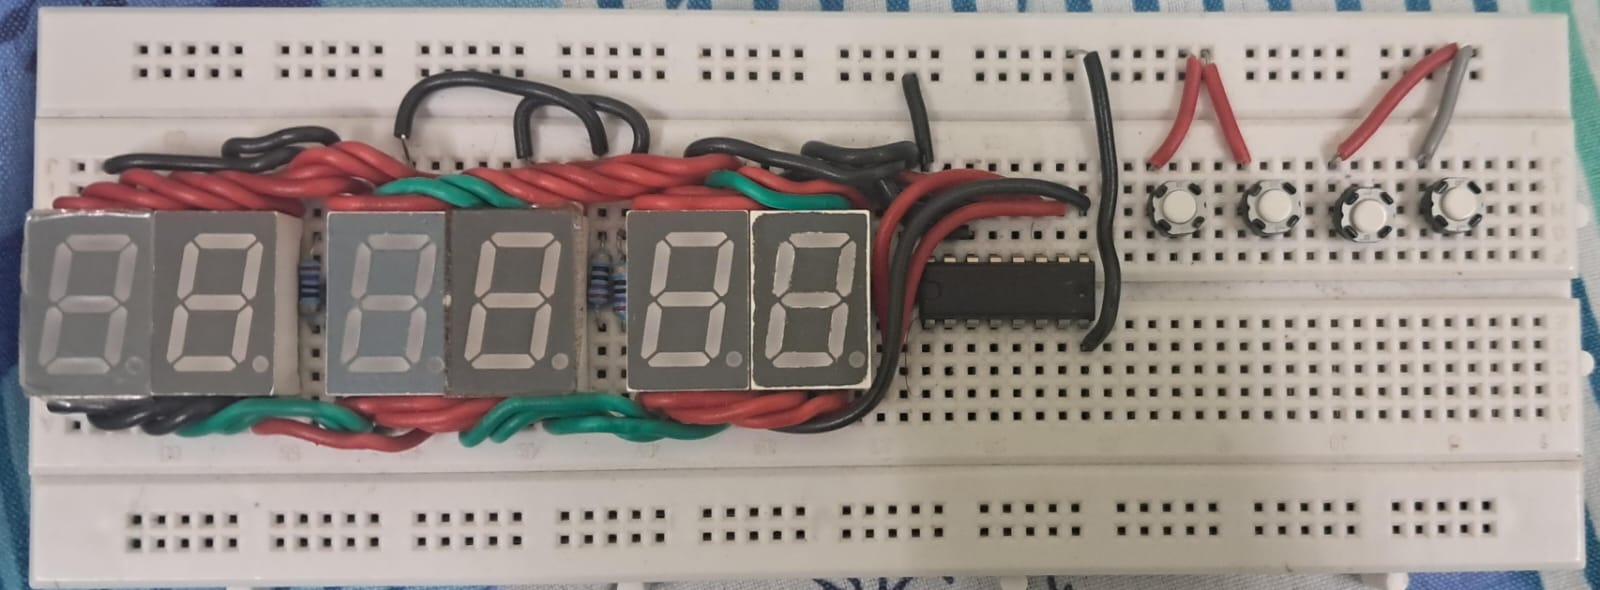
\includegraphics[width=0.5\textwidth]{figs/clock.jpeg}
\centerline{Figure 1 - Final Clock}

\end{document}
